\documentclass{article}
\usepackage[utf8]{inputenc}
\usepackage{amsmath, amssymb, multicol, enumerate, tikz}
\usepackage[margin = 0.5in]{geometry}
\pagestyle{empty}
\raggedright
\newcounter{PS}
\begin{document}

Name \makebox[3in]{\hrulefill} \hfill Honors Algebra 2 PSet

\subsubsection*{Compound Inequalities \hfill \makebox[0.35in]{\hrulefill} / 10}

Solve each of the following and graph your solution on a number line.
\begin{flalign*}
1. \quad    &		6 < x + 3 < 8		&
2. \quad	&	-3 \leq x+2 < 1	&&\\[2in]
3. \quad	&	-6 \leq \dfrac{x}{2} - 4 < -3	&
4. \quad	&	-11 < 2x-1 \leq -5	&&\\[2.25in]
5. \quad	&	3x>12 \text{ or } 2x<-6	&
6. \quad	&	2x-5 \leq -11 \text{ or } 5x+1 \geq 6	&&\\[2.25in]
7. \quad	&	2x+1 < 15 \text{ or } 3x-4 \geq -1		&
8. \quad	&	-2x+5>7 \text{ or } -3x+10>2x		&&\\
\end{flalign*}

\newpage

\subsection*{Compound Inequalities Answers}

\begin{enumerate}
    \item $3 < x < 5$   \\[0.15in]
    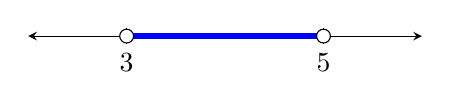
\begin{tikzpicture}
    \draw [<->, >=stealth] (-2.5,0) -- (2.5,0);
    \draw (-1.25,0.1) -- (-1.25,-0.1);
    \draw (1.25,0.1) -- (1.25,-0.1);
    \node at (-1.25,-0.1) [anchor=north] {$3$};
    \node at (1.25,-0.1) [anchor=north] {$5$};
    \draw [color=blue, line width=2] (-1.25,0)--(1.25,0);
    \draw [fill=white] (-1.25,0) circle (2.5pt);
    \draw [fill=white] (1.25,0) circle (2.5pt);
    \end{tikzpicture}
    
    \item $-5 \leq x < -1$  \\[0.15in]
    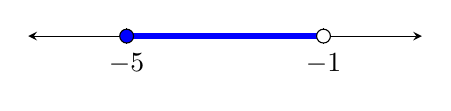
\begin{tikzpicture}
    \draw [<->, >=stealth] (-2.5,0) -- (2.5,0);
    \draw (-1.25,0.1) -- (-1.25,-0.1);
    \draw (1.25,0.1) -- (1.25,-0.1);
    \node at (-1.25,-0.1) [anchor=north] {$-5$};
    \node at (1.25,-0.1) [anchor=north] {$-1$};
    \draw [color=blue, line width=2] (-1.25,0)--(1.25,0);
    \draw [fill=blue] (-1.25,0) circle (2.5pt);
    \draw [fill=white] (1.25,0) circle (2.5pt);
    \end{tikzpicture}    
    
    \item $-4 \leq x < 2$   \\[0.15in]
    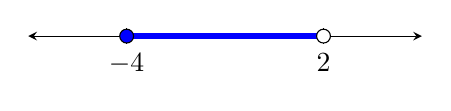
\begin{tikzpicture}
    \draw [<->, >=stealth] (-2.5,0) -- (2.5,0);
    \draw (-1.25,0.1) -- (-1.25,-0.1);
    \draw (1.25,0.1) -- (1.25,-0.1);
    \node at (-1.25,-0.1) [anchor=north] {$-4$};
    \node at (1.25,-0.1) [anchor=north] {$2$};
    \draw [color=blue, line width=2] (-1.25,0)--(1.25,0);
    \draw [fill=blue] (-1.25,0) circle (2.5pt);
    \draw [fill=white] (1.25,0) circle (2.5pt);
    \end{tikzpicture}    
    
    \item $-5 < x \leq -2$  \\[0.15in]
    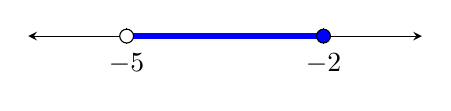
\begin{tikzpicture}
    \draw [<->, >=stealth] (-2.5,0) -- (2.5,0);
    \draw (-1.25,0.1) -- (-1.25,-0.1);
    \draw (1.25,0.1) -- (1.25,-0.1);
    \node at (-1.25,-0.1) [anchor=north] {$-5$};
    \node at (1.25,-0.1) [anchor=north] {$-2$};
    \draw [color=blue, line width=2] (-1.25,0)--(1.25,0);
    \draw [fill=white] (-1.25,0) circle (2.5pt);
    \draw [fill=blue] (1.25,0) circle (2.5pt);
    \end{tikzpicture}     
    
    \item $x>4$ or $x<-3$   \\[0.15in]
    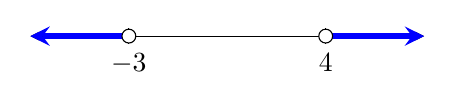
\begin{tikzpicture}
    \draw [<->, >=stealth] (-2.5,0) -- (2.5,0);
    \draw (-1.25,0.1) -- (-1.25,-0.1);
    \draw (1.25,0.1) -- (1.25,-0.1);
    \node at (-1.25,-0.1) [anchor=north] {$-3$};
    \node at (1.25,-0.1) [anchor=north] {$4$};
    \draw [->, >=stealth, color=blue, line width=2] (-1.25,0)--(-2.5,0);
    \draw [->, >=stealth, color=blue, line width=2] (1.25,0)--(2.5,0);
    \draw [fill=white] (-1.25,0) circle (2.5pt);
    \draw [fill=white] (1.25,0) circle (2.5pt);
    \end{tikzpicture} 
    
    \item $x\leq-3$ or $x\geq 1$    \\[0.15in]
    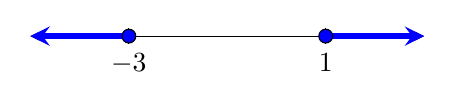
\begin{tikzpicture}
    \draw [<->, >=stealth] (-2.5,0) -- (2.5,0);
    \draw (-1.25,0.1) -- (-1.25,-0.1);
    \draw (1.25,0.1) -- (1.25,-0.1);
    \node at (-1.25,-0.1) [anchor=north] {$-3$};
    \node at (1.25,-0.1) [anchor=north] {$1$};
    \draw [->, >=stealth, color=blue, line width=2] (-1.25,0)--(-2.5,0);
    \draw [->, >=stealth, color=blue, line width=2] (1.25,0)--(2.5,0);
    \draw [fill=blue] (-1.25,0) circle (2.5pt);
    \draw [fill=blue] (1.25,0) circle (2.5pt);
    \end{tikzpicture}     
    
    \item All Real Numbers $(\mathbb{R})$   \\[0.15in]
    
\begin{tikzpicture}
    \draw [<->, >=stealth] (-2.5,0) -- (2.5,0);
    \draw (0,0.1) -- (0,-0.1);  
    \draw [<->, >=stealth, color=blue, line width=2] (-2.5,0)--(2.5,0);
    \end{tikzpicture}
    
    \item $x<2$    \\[0.15in]
    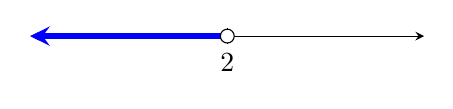
\begin{tikzpicture}
    \draw [<->, >=stealth] (-2.5,0) -- (2.5,0);
    \draw (0,0.1) -- (0,-0.1);  
    \node at (0,-0.1) [anchor=north] {$2$};
    \draw [->, >=stealth, color=blue, line width=2] (0,0)--(-2.5,0);
    \draw [fill=white] (0,0) circle (2.5pt);
    \end{tikzpicture}    
\end{enumerate}

\end{document}
